\chapter{Implementazione Rsa in Gnuradio}
\label{cha:999}
La seconda parte del lavoro svolto è stata qualla di valutare la possibilità dell'aggiunta di una criptografia RSA al sistema di trasmissione OFDM. Il primo passo è stato sviluppare un modulo che criptasse le informazioni passando poi all'implementazione di un secondo blocco per la decodifica. Le chiavi utilizzate non sono assolutamente sicure, sono state scelte piccole solo per rendere facile la comprensione e seguire il funzionamento. In un applicazione reale sono necessarie chiavi di almeno 1024bit.
\section{Sviluppo dei moduli}
Lo sviluppo dei moduli è diviso in tre parti fondamentali descritte in seguito, per la creazione dei file di supporto e l'importazione delle librerie necessarie Gnuradio mette a disposizione un tool chiamato gr\_moodtool utilizzabile da riga di comando.
\subsection{Definizione proprietà moduli per l'ambiente grafico}
Di seguito sono mostrati i file contenenti la definizione dei parametri necessari per l'interazione con l'ambiente. I blocchi sono costituiti da un ingresso per ricevere il flusso dati dal programma "Sink" ed un uscita per permettere la continuazione "Source", inoltre possono richiedere parametri aggiuntivi che devono essere forniti dall'utente nel formato corretto.
Al codificatore è richiesto sapere la coppia di valori che costituiscono la chiave pubblica del decodificatore mentre per la decriptazione è sufficiente la chiave privata.
\begin{figure}[h]
	\centering
	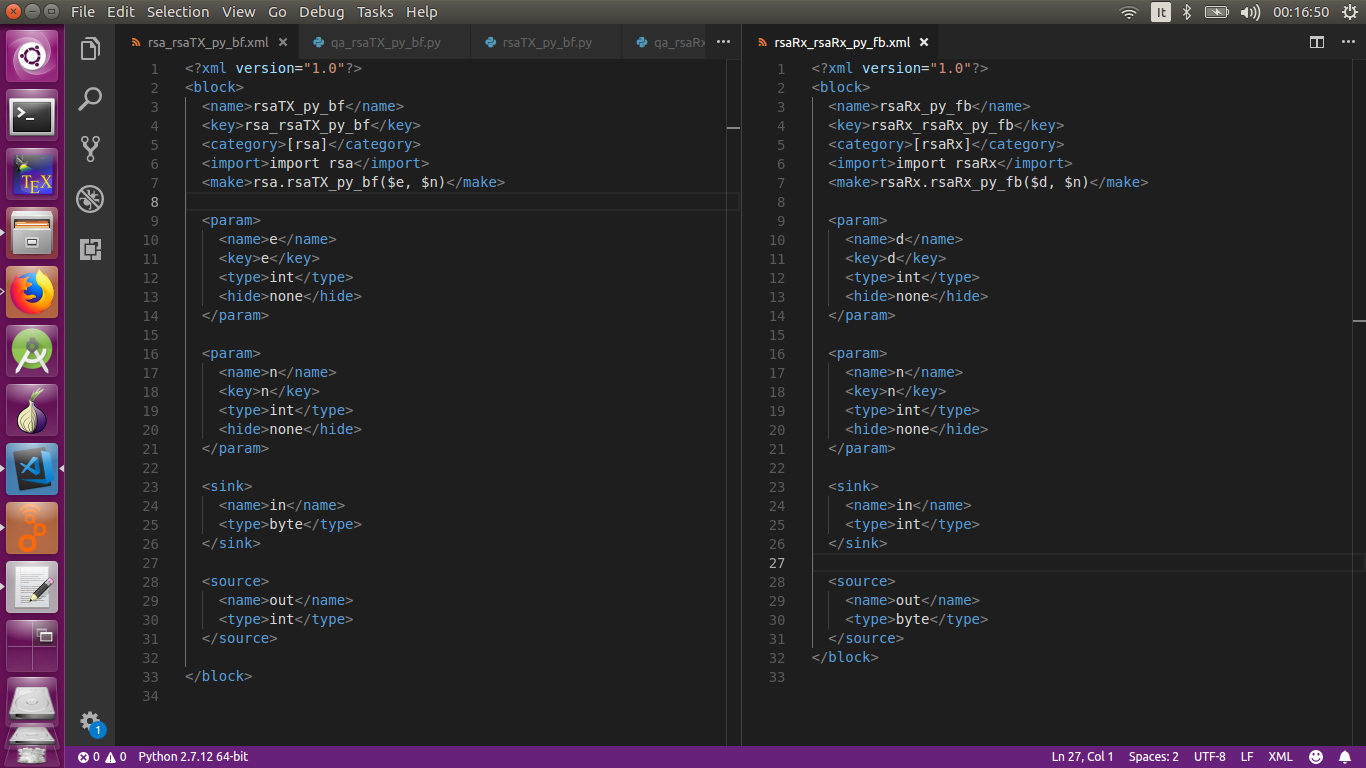
\includegraphics[scale=0.35]{rsaXml}
	\caption{File contenenti la definizione dei parametri nell' ambiente grafico}
\end{figure}
\subsection{Algoritmo per cifratura e decifratura}
La codifica e la decodifica rsa si effettua utilizzando lo stesso algoritmo e fornendo la chiave corretta. Nell'implementazione di rsa è importante non effettuare subito l'elevamento a potenza in quanto può originare numeri enormi, l'approccio migliore consiste nel  moltiplicare la base n volte calcolando il modulo ad ogni passaggio.
Il collegamento logico fra i blocchi all'interno dell'ambiente gnuradio al momento dell'esecuzione viene tradotto in un file python il cui compito è quello di gestire il flusso delle informazioni istanziando le classi dei blocchi necessari e successivamente chiamare il loro metodo "work" presente in ogni modulo.
 Lo sviluppo del proprio algoritmo deve essere implementato proprio all' interno della funzione work.
 Le informazioni vengono trasferite attraverso un vettore di vettori. il primo indice rappresenta la numerazione dell'ingresso o dell'uscita mentre il secondo permette di gestire l'arrivo di più informazioni alla volta.
\begin{figure}[h]
	\centering
	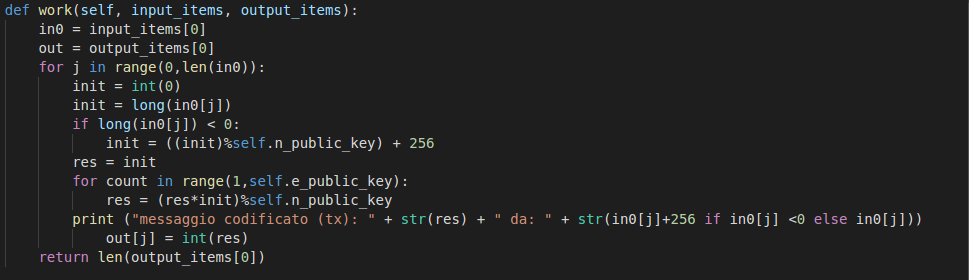
\includegraphics[scale=0.40]{rsaTxCode}
	\caption{Algoritmo per il blocco di codifica}
\end{figure}
Il blocco codificatore riceve 8 bit alla volta che vengono tradotti in python con il complemento a due. il risultato della cifrazione non risulta più rappresentabile con 8bit e per la nostra analisi di fattibilità effettuata con chiavi deboli è stato sufficiente l'utilizzo di una variablile intera. L'applicazione in uno scenario reale implica la risoluzione di problematiche discusse nella sezione delle conclusioni.
\begin{figure}[h]
	\centering
	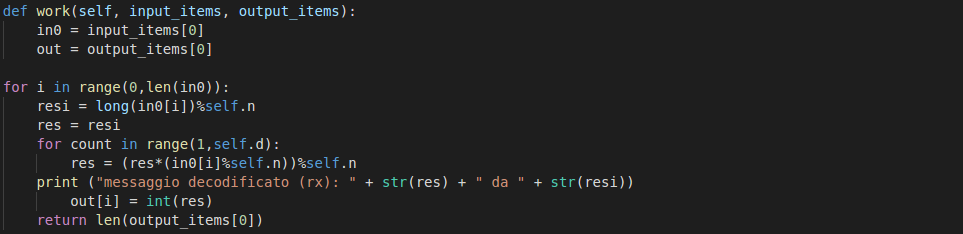
\includegraphics[scale=0.40]{rsaRxCode}
	\caption{Algoritmo per il blocco di decodifica}
\end{figure}
Il blocco Decodificatore riceve le informazioni codificate e le riporta nel formato originale.
\subsection{Codice di test}
Gnuradio permette la creazione di casi di test come spiegato nella sezione di introduzione teorica, il testing è particolarmente utile in scenari come quello presente dove un eventuale errore nell'algoritmo verrebbe propagato ai blocchi successivi senza produrre segnalazioni. Le funzioni di testing sono utili anche durante lo sviluppo in quanto permettono di provare il codice scritto senza dover compilare tutto il modulo per renderlo disponibile nell'ambiente Gnuradio. Il testing viene effettuato istanziando la classe del blocco in analisi collegandolo ad una sorgente dati che si occuperà di passare i dati specificati ed un pozzo per riceverli una volta processati. Vengono inoltre impostati i parametri richiesti dal modulo(nel nostro caso riguardano i due valori di cui sono composte le chiavi). Infine vengono confrontati i risultati utilizzando delle funzioni apposite dette "assert" che restituiscono un messaggio di errore se falliscono.
Nel testing del blocco di codifica i valori scelti (128,255,0,7,127) coprono tutti i casi limite del complemeto a due.
\begin{figure}[h]
	\centering
	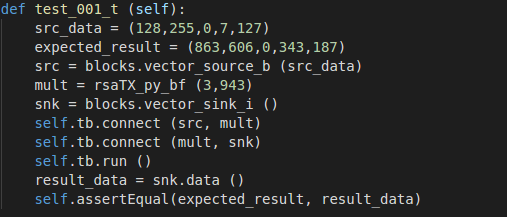
\includegraphics[scale=0.40]{rsaTxQa}
	\caption{Codice di test per il bocco di codifica}
\end{figure}
\subsection{Importazione in Gruradio}
Il passo finale consiste nel compilare i moduli e farli funzionare nell'ambiente grafico Gnuradio. Nella console inclusa in basso nell'interfaccia utente vengono stampati dei feedback generati dai moduli durante il loro lavoro. L'esempio riportato trasferisce un testo cifrandolo. Questo modello non è tuttavia ancora applicabile ad una comunicazione reale per le motivazioni discusse nelle conclusioni.
\begin{figure}[h]
	\centering
	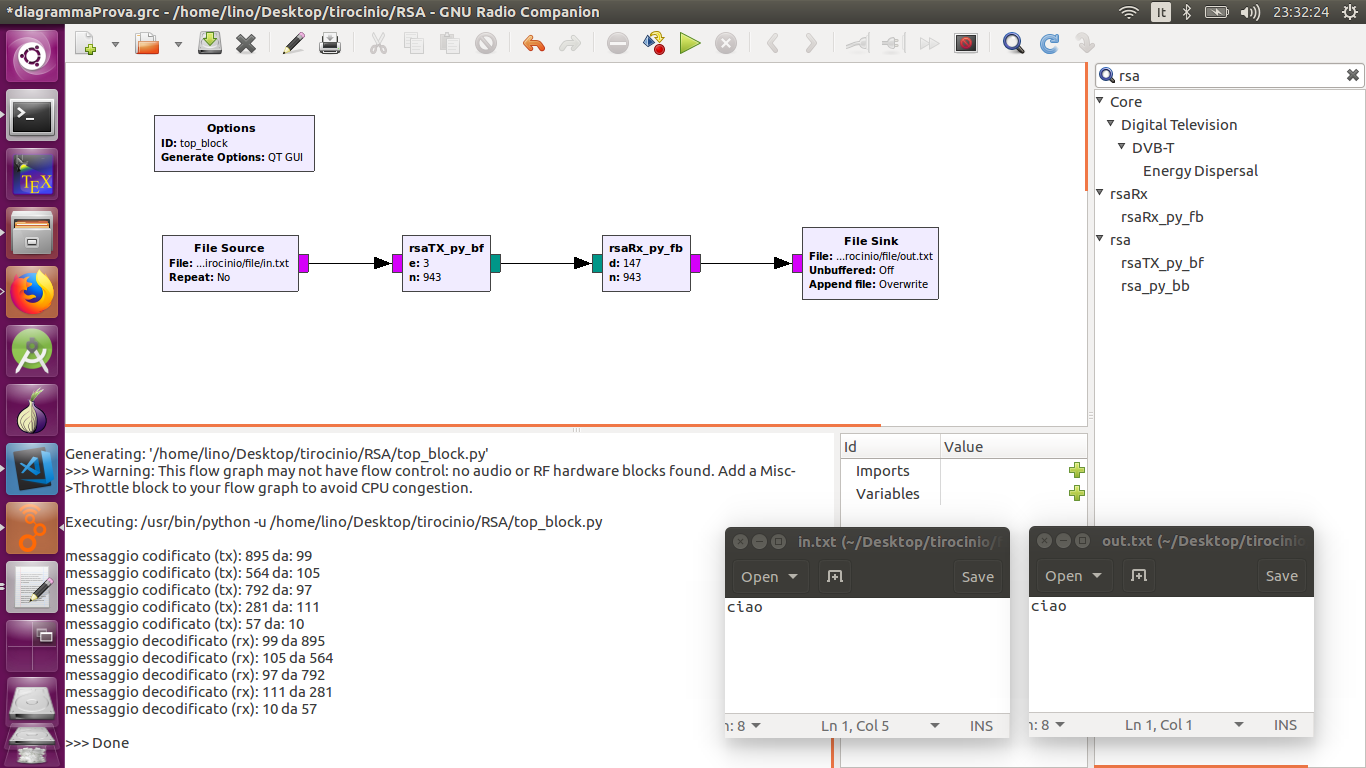
\includegraphics[scale=0.35]{rsaSimulazione}
	\caption{Codice di test per il bocco di codifica}
\end{figure}

\newpage
